\input{header}

\AtBeginSubsection[]
{
	\begin{frame}<beamer>
		\frametitle{Outline}
		\tableofcontents[current,currentsubsection]
	\end{frame}
}

\begin{document}

\begin{frame}[allowframebreaks] \frametitle{Example 2.16}

  \begin{equation*}
  \{a^i b^j c^k
\mid i=j \mbox{ or } i = k\}
\end{equation*}
  \begin{itemize}
\item Idea: push $a^i$ into stack

\item [] But should we check $b$ or $c$ ?

\item Need \alert{nondeterminism}
\item Pushdown automata may be nondeterministic
\item Recall $\delta$ was defined as
    \begin{equation*}
  Q \times 
\Sigma_{\epsilon} \times \Gamma_{\epsilon}
\rightarrow P(Q\times \Gamma_\epsilon)
\end{equation*}
We see the power set $P(Q\times \Gamma_\epsilon)$ 
\item Fig 2.17
\item [] The upper part checks if $i=j$
\item [] The lower part checks if $i=k$
\end{itemize}

\scalebox{0.9}{
\begin{tikzpicture}
\node[state,initial] (q_1) {$q_1$};
\node[state] (q_2) [right of=q_1] {$q_2$};
\node[state] (q_3) [above right of=q_2] {$q_{3}$};
\node[state,accepting] (q_4) [right of=q_3] {$q_{4}$};
\node[state] (q_5) [below right of=q_2] {$q_{5}$};
\node[state] (q_6) [right of=q_5] {$q_{6}$};      
\node[state,accepting] (q_7) [right of=q_6] {$q_{7}$};      

\path 
(q_1) edge[above]  node {$\epsilon, \epsilon \rightarrow \$ $} (q_2)
(q_2) edge[loop above]  node {$a,\epsilon \rightarrow a$} (q_2)
(q_2) edge[right]  node {$\epsilon, \epsilon \rightarrow \epsilon$} (q_3)
(q_2) edge[right]  node {$\epsilon, \epsilon \rightarrow \epsilon$} (q_5)
(q_3) edge[loop above]  node {$b, a \rightarrow \epsilon$} (q_3)
(q_3) edge[above]  node {$\epsilon, \$ \rightarrow \epsilon$} (q_4)
(q_4) edge[loop above]  node {$c, \epsilon \rightarrow \epsilon$} (q_4)
(q_5) edge[loop below]  node {$b, \epsilon \rightarrow \epsilon$} (q_5)
(q_5) edge[below]  node {$\epsilon, \epsilon \rightarrow \epsilon$} (q_6)
(q_6) edge[loop below]  node {$c, a \rightarrow \epsilon$} (q_6)
(q_6) edge[below] node {$\epsilon, \$ \rightarrow \epsilon$} (q_7);
  \end{tikzpicture}
}

\begin{itemize}
\item nondeterminism: $q_2 \rightarrow q_3$
or $q_2 \rightarrow q_5$

and others ($q_5 \rightarrow q_5
$ or $q_5 \rightarrow q_6$)

one for $b^i$ and one for $c^i$

\item Exercise: $a^2bc^2$ (a tree)

  
\end{itemize}\end{frame}

\begin{frame}[allowframebreaks]
  \frametitle{Running a PDA}
  \begin{itemize}
  \item Input $a^2bc^2$
  \item The way is similar to how we run an NFA
\end{itemize}
  
  \begin{center}
\scalebox{0.9}{    
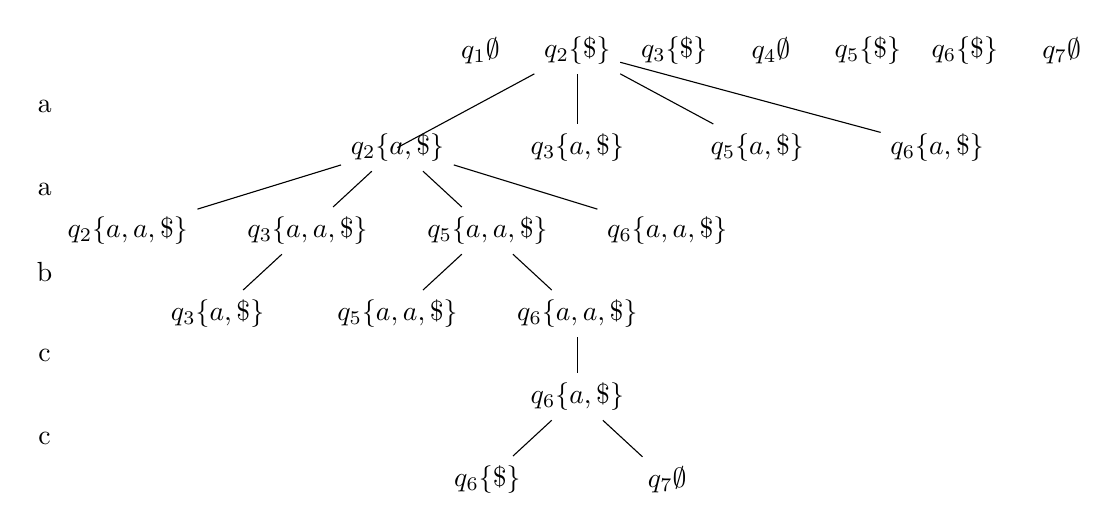
\begin{tikzpicture} [level distance=25pt,sibling distance=65pt]% grow=right
\node  {$q_1\emptyset$}
child [grow=right, level distance=35pt] { node  { $q_2\{\$\}$ } edge from parent[draw=none]
  [grow=down]
  child [grow=right] { [level distance=35pt] node  {$q_3\{\$\}$} edge from parent[draw=none]
    child [grow=right] {node  {$q_4\emptyset$} edge from parent[draw=none]
      child [grow=right] {node  {$q_5\{\$\}$} edge from parent[draw=none]
        child [grow=right] {node  {$q_6\{\$\}$} edge from parent[draw=none]
          child [grow=right] {node  {$q_7\emptyset$} edge from parent[draw=none]
          }
        }
      }
    }
  }
  child { [level distance=30pt] node  {$q_2\{a,\$\}$}
    child {node  {$q_2\{a,a,\$\}$}
      child [grow=left] {node (3) {} edge from parent[draw=none]
        child [grow=up] {node (2) {} edge from parent[draw=none]
          child [grow=up] {node (1) {} edge from parent[draw=none]
          }
        }
        child [grow=down] {node (4) {} edge from parent[draw=none]
          child [grow=down] {node (5) {} edge from parent[draw=none]
            child [grow=down] {node (6) {} edge from parent[draw=none]
            }
          }
        }
      }
    }
    child {node  {$q_3\{a,a,\$\}$}
      child {node  {$q_3\{a,\$\}$}
      }
      child {edge from parent[draw=none]}      
    }
    child {node  {$q_5\{a,a,\$\}$}
      child {node  {$q_5\{a,a,\$\}$}}
      child {node  {$q_6\{a,a,\$\}$}
        child {node  {$q_6\{a,\$\}$}
          child {node  {$q_6\{\$\}$}}
          child {node  {$q_7\emptyset$}}
        }
      }
    }
    child {node  {$q_6\{a,a,\$\}$}}
  }    
  child  {node {$q_3\{a,\$\}$}}      
  child  {node {$q_5\{a,\$\}$}}
  child  {node {$q_6\{a,\$\}$}}
};
\path (1) -- (2) node [midway] {a};
\path (2) -- (3) node [midway] {a};
\path (3) -- (4) node [midway] {b};
\path (4) -- (5) node [midway] {c};
\path (5) -- (6) node [midway] {c};
\end{tikzpicture}
}
\end{center}
\end{frame}

\begin{frame}[allowframebreaks] \frametitle{Example 2.18}
  \begin{itemize}
\item $\{ww^R\mid w \in \{0,1\}^*\}$

\item [] $w^R$: reverse
\item Approach:

\item [] symbols pushed to stack

\item [] nondeterministically guess middle is reached


\item fig 2.19

\begin{center}
\begin{tikzpicture}
\node[state,initial,accepting] (q_1) {$q_1$};
\node[state] (q_2) [right of=q_1] {$q_2$};
\node[state] (q_3) [below of=q_2] {$q_{3}$};
\node[state,accepting] (q_4) [left of=q_3] {$q_{4}$};      
  \path 
  (q_1) edge[above]  node {$\epsilon, \epsilon \rightarrow \$ $} (q_2)
  (q_2) edge[loop right]  node {
    \begin{tabular}{l}
      $0,\epsilon \rightarrow 0$\\
      $1,\epsilon \rightarrow 1$
    \end{tabular}
} (q_2)
  (q_2) edge[right]  node {$\epsilon, \epsilon \rightarrow \epsilon$} (q_3)
  (q_3) edge[loop right]  node {
    \begin{tabular}{l}
      $0, 0 \rightarrow \epsilon$
      \\
      $1, 1 \rightarrow \epsilon$
    \end{tabular}
} (q_3)  
  (q_3) edge[below] node {$\epsilon, \$ \rightarrow \epsilon$} (q_4);
  \end{tikzpicture}
\end{center}

  
\end{itemize}\end{frame}
\end{document}
